\documentclass[a4paper, 12pt, notitlepage]{report}

\usepackage{amsfonts} % if you want blackboard bold symbols e.g. for real numbers
\usepackage{graphicx} % if you want to include jpeg or pdf pictures
\setcounter{secnumdepth}{5}

\title{{\Huge Modelling Project} \vspace{300pt}} % change this
\author{Yoram Meijaard\\Chiel van Horssen\\Youri Haenen\\Bram Maas\\Martijn Ras\\Sascha Worms} % change this
\date{\today} % change this

\begin{document}

%%%%%%%%%% PRELIMINARY MATERIAL %%%%%%%%%%
\maketitle
\begin{center}
The report on the wheelchair problem of airline companies % change this
\\[12pt]
Supervised by: I. Papaliouras  % change this
\end{center}
\thispagestyle{empty}
\newpage
% \section*{Acknowledgement of Sources} % this must be included in undergradate projects
% For all ideas taken from other sources (books, articles, internet), the source of the ideas is mentioned in the main text and fully referenced at the end of the report.

% All material which is quoted essentially word-for-word from other sources is given in quotation marks and referenced.

% Pictures and diagrams copied from the internet or other sources are labelled with a reference to the web page or book, article etc.
% \\[12pt]
% Signed \dotfill Date \dotfill

\tableofcontents

%%%%%%%%%% MAIN TEXT STARTS HERE %%%%%%%%%%

%%%%%%%%%% SAMPLE CHAPTER %%%%%%%%%%
% \chapter{Summary}

% \chapter{Description of modeling process}

%first deadline
\chapter{Definition phase}
\section{Context}
\subsection{The Stakeholders and the keydrivers }
The stakeholders are:
\begin{itemize}
 \item KLM
 \item Escorts
 \item Passengers
 \item Employees
 \item Other airline companies and other airport
 \item  constructors and maintainers of the wheelchairs.
\end{itemize}
These person have got the greatest interest in the escort service in general, including if the service was optimized to be efficient in time and thus in costs. The people who guard the depot where the wheelchairs are stored and desk workers who check in the passengers are both taken into account in the employees. The keydrivers are:
\begin{itemize}
	\item Efficiency
	\item Cost
	\item Optimization
	\item Comfort
	\item Time
	\item Safety
	\item Reliability
\end{itemize}
\subsection{Relation between the stakeholders and keydrivers}
If the Stakeholders are linked to the keydrivers, their relations could be summarized into this mind map:
\begin{center}
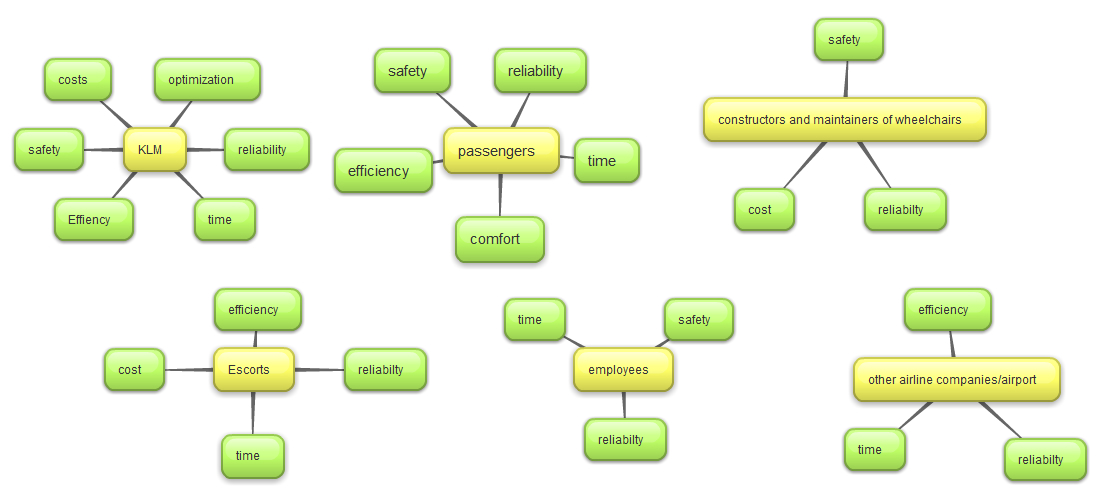
\includegraphics[scale=0.4]{figures/relationstakeholders.jpg}
\end{center}
\subsubsection{KLM}
One of the interests of KLM is the costs to keep them as low as possible, but not such that this is the main interest. The plane needs to leave on time, so there needs to be a minimum amount of money to realize the on time depart of the plane.\\
Safety is another interest, which deals with the safety of the escort service. This deals then with the safety of the trip, the safety of the wheelchairs etc. If the safety is not of a certain level, such that the reputation of the airline company suffers, people might rather use other airline companies to realize their trip.\\
The same reason holds for efficiency. Also, if the service is not efficient, not as many escorts by the same person can be taken care of, so the plane might leave late. Therefore an efficient solution with respect to time needs to be archived.\\
So as mentioned above, time is also a factor which is required to keep costs low and hence a high efficiency as result. The distance from the check-in desk to the gate can be considered in time for example.\\
Reliability of the service also deals with the safety reasons: KLM needs to be sure the service takes a certain time and it should be sure that the passengers arrive on time at the gate. Unreliable service leads to loss of money and reputation damage.\\
Finally, optimization is the most important interest for KLM, so the service gets optimized to cost minimally but that the plane can depart on time.
\subsubsection{Escorts}
The costs are also important for the escort itself. If the costs are getting too high, the might be a possibility that these people are fired or a drop in wage. So indirectly they have an interest in the costs of their service.\\
With respect to the efficiency, which is also a keydriver for the escorts, time is important. This relates to the costs (as mentioned above), because the more escorts executed, the more employees are required to perform all escorts, which means higher costs, hence in contradiction with the main goal. \\
Reliability is required by the escort, such KLM can assure the passengers that they will be on time at the gate, so again also to keep costs low. On the other hand, other personnel of the service needs to be sure that certain staff is at position x at time t, so efficiently using the resources and personnel of the service to optimize the service.\\
Efficiency follows then directly from the above mentioned relations in order to keep costs low of the service.
\subsubsection{Passengers}
The passengers are interested in having a comfortable, safe, efficient and reliable escort. Comfort can be archived by having a sufficient comfortable ride and wheelchair used to transport the person from the desk to the gate. Since the passenger does not want to see the whole airport,  time is also in the interest of the passengers. This also relates to efficiency: the disabled passenger wants to be escorted in the shortest possible time, with as much comfort as possible. This means that some  is required and hence the service needs to be efficient. \\
The reliability is of interest for the passengers, by the fact that
the passenger wants to be sure to get the escort when request, which in generally happens. Also, the passenger want to be brought to a specific gate, at a specific time. Therefore the reliability of the escort service is also of interest for the passengers.\\
Finally, safety is also of interest, because the passenger wants to be escorted safely without injuries. Therefore the wheelchair needs to be safe to be used, and the quality of service of the escort needs to be of a certain level. This level requires a certain level of service from the personnel.
\subsubsection{Employees}
The interest of the employees, are the time (duration of the escort), reliability and the safety of the escort. The time is of interest, because of the fact that when a transfer has to be made, the escort is on time at the gate to get the passenger and is on time at the next gate to board the passenger such that the next plane (also) can leave on time. The employees guarding the depot on the other hand have got an interest in time as well. Their interest is to know how long a wheelchair is away from the depot, but also to be able to check if something happened with the escort or the wheelchair (i.e. lost or accident). \\
Safety is also of concerns of the employees, since if the goal of an airline company is to maintain quality and safety, all employees should be able to contribute in their way. The escorting persons therefore need to make sure the escorted person is moved safely from place A to place B.
\subsubsection{Constructors and maintainers of the wheelchairs}
The maintainers and constructors of the wheelchairs have interest in the safety, costs and reliability. They have to make sure the wheelchair is safe,  in usage for both the disabled person and the escort service. The escort service could get a bad reputation if the escort service is not safe.\\
On the other hand, the costs should not be too high. So the people have to construct and maintain the wheelchairs in such a way to create good wheelchairs with not too high costs (both maintenance and product price). But the demand for low costs is opposed by the safety of the wheelchairs. If the construction is not solid enough so any\footnote{Obviously not everyone should be taken into account, but i.e. obese people need tougher wheelchairs, hence some 'extremes' need to be taken care of in the construction, but not all.} possible disabled person can be transferred safely. So the wheelchair also needs to be sufficiently solid built.
\subsubsection{Other airline companies and other airports}
Other airline companies and other airports also have an interest in the escort service in the following perspective. If the transfer is a transfer between two different planes of different airline companies\footnote{Only from KLM to airline company X is considered}, the other company requiers a time efficient, reliable escort service such that this plane can depart on time.\\
In the worst case, there is little time between arrival of plane 1 and depart of plane 2. A time efficient service would be necessary to realize this. Also an estimation on when a disables person with escort arrives is pleasant to know when an escort approximately arrives. Clearly, this should be as efficient as possible and hence efficiency is also an interest.\\
Reliability is also an interest for other airline companies and airports. Being sure when an escort arrives is necessary in order to make it possible for other airline companies to depart on time when there is a transfer with escort service. If it is uncertain if the passenger will arrive on time, it is cheaper for an airline company to let the plane depart and put the escorted person on a plane departing later than to miss the timeslot in which the plane was supposed to leave with all (worse) economic consequences as result. Therefore reliability of the escort service is also of interest for other aiports and other airline companies.
\newpage
\subsection{Relation between keydrivers}
The keydrivers do also have a relation with other keydrivers than only with stakeholders. These can be summarized as follows:
\begin{center}
	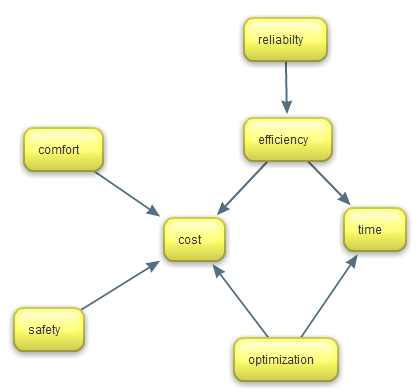
\includegraphics[scale=0.45]{figures/relationkeydrivers.jpg}
\end{center}
The arrows should be read that keydriver $k$ has in incoming arrow from $k'$, and $k'$ has and incoming arrow from $k"$, $k$ is in a relation with $k"$. So there is transitivity between the elements.
\subsubsection{Reliability}
In order to have a reliable service, so the service is on time and there are no losses of money on the service, it can be said that reliability is linked to both cost and time in the respect of efficiency. Therefore by transitivity reliability is related to efficiency.
\subsubsection{Efficiency}
As stated by reliability, the costs should not be low and the escort should be time efficient. So in general the service needs to be both efficient in time and costs. Therefore efficiency has a relation with both cost and time.
\subsubsection{Optimization}
So both time and cost should be in relation with optimization. The cost should be kept as low as possible to give an time efficient reliable service. But then there should be optimization on time with costs reduction as a result\footnote{Compared to the case where no attention has been paid to optimized model where planes leave late with all financial consequences as result}. Therefore there needs to be a relation from optimization to both cost and time.
\subsubsection{Safety}
When safety is addressed, money is always a factor. Safety costs money, and the level of safety sets the costs in order to realize. If for example the wheelchair needs to be made that it has bumpers to take the impact and not the one sitting in the wheelchair. But this costs money to realize. This shows the direct relation between safety and cost, which therefore exists.
\subsubsection{Comfort}
The comfort also relates to money in the same respect as safety does. If the transported person is transported in a very relaxing wheelchair, then this wheelchair costs more money than a plain wheelchair. If the ride to the gate is desired to be more comfortable, then the duration needs to be longer which as a result costs more money. Hence, comfort is in a relation with cost.
%%%%%%%%%%%%%%%%%%%%%%%%%%%%%%%%%%%%%%%%%%%%%%%%%%%%%%%%%%%%%%%%%%%%%%%%%%%%%%%%%%%%%%%%
\section{Problem definition and purpose}
\subsection{Model purpose}
When making a model there should be three questions answered:\\
\emph{Is there something to choose?\\
Will the model output a number?\\
Should the model produce a value or knowledge?}\\\\
The first question can be answered with \emph{yes}, that is because there are different combinations for different sets of people, area ect.\\
The second question will also be answered with \emph{yes} since the model should produce a number of escorts or wheelchairs needed so the cost can be calculated.\\
The answer to the last question should be a \emph{value}, because the model brings an optimized solution rather than new knowlage.\\ From this we can conclude the model should be a \emph{optimization}, it should produce the best solution possible for the owner.
\subsection{Model dimensions}
Now that the purpose of the model is known, the dimensions should be determined. This can be done using the following points.
\subsubsection{Continue or discrete}
The model should be a \emph{discrete} model, since all input and output values are integers, also most of the intermediate results will be discrete numbers.
\subsubsection{Deterministic or stochastic}
Since the owner of the model can decide almost all input variables, the assumption is that this model is \emph{deterministic}. The owner has influence on most of the inputs, and also the number of wheelchairs and disabled people will be deterministic.
\subsubsection{Black box or glass box}
The model will be a \emph{glass box} model, because there is insight in what happens, everything is known by the owner of the model, for instance the owner knows how many disabled people travel and where and when planes arrive and leave.
\subsubsection{Static or dynamic}
Because time does not matter -the model is, after all, just about one transfer- this is a \emph{static} model. All input values are set before execution and are valid throughout the entire model.
\subsubsection{Calculating or reasoning}
The model will be a \emph{calculating} model, because a number is the desired output of the model. Also all input values and quantities will be numbers.
\subsubsection{Geometrical or non-geometrical}
Even though an airport feels like a geometric setting the model is a \emph{non-geometrical} model, this is because the airport will not be geographically defined, there are only distances used which are abstract numbers.
\subsubsection{Numerical or symbolic}
It is not entirely clear whether the model is numerical or symbolic since the model itself starts out using only symbols for the inputs in the formulas, but once executed the the model will replace these with concrete values, also the output will be numerical. This makes the model \emph{both numerical and symbolic}.
\subsubsection{Material or immaterial}
The model will be \emph{Immaterial}, because the model does not describe a real airport. There is just a concept in our mind that we project into this immaterial model. It will sort of look like modeling from scratch, but with a discrete model.
\subsection{Conceptual definition of the problem}
Given a description of the airport, incoming flights and departing flights: how many resources are required to get all flights of the ground with all immobile people on board?
\section{Sub-questions}
\begin{enumerate}
\item How will the number of wheelchairs influence the amount of time of a transfer between two flights?
\item How will the location of the wheelchair depot influence the time?
	\begin{enumerate}
	\item What will this mean for the distance between the gates?
	\item What will this mean for the time required to travel between to gates?
	\item What will this mean for the maintenance of the wheelchairs
		\begin{enumerate}
		\item Who will do the maintenance of the wheelchairs?
		\item How much service does each wheelchair require?
		\item Where will those wheelchairs be bought?
		\end{enumerate}
	\item How will this influence the amount of escorts?
		\begin{enumerate}
		\item How many escorts do I need for one wheelchair?
		\end{enumerate}
	\item Will the storing of the chairs at one location decrease the costs of guarding them?
		\begin{enumerate}
		\item Will hiring additional security to guard the wheelchairs result in less damage/stolen chairs?
		\item If the escorts guard the chairs, how will this influence security?
			\begin{enumerate}
			\item Do we have to hire more escorts if they handle security?
			\end{enumerate}
		\end{enumerate}
	
	\end{enumerate}
\item What kind of wheelchairs will be used?
	\begin{enumerate}
	\item Will the quality of the chair influence the amount of maintenance required?
	\item Will the quality of the chair influence the amount of money asked for the service?
	\item How will the quality of the wheelchair influence the customer satisfaction?
		\begin{enumerate}
		\item How will this distinct KLM from other airliners?
		\item Will this create an increase in customers?
		\end{enumerate}
	\item Which wheelchair has the best price/quality rate?
		\begin{enumerate}
		\item How much is the difference in price?
			\begin{enumerate}
			\item How will the difference in price influence the total costs?
			\item What is the price of each wheelchair?
			\end{enumerate}
		\end{enumerate}
	\end{enumerate}
\item How will the amount of escorts influence the total costs?
	\begin{enumerate}
	\item What kind of people will escort the disabled?
		\begin{enumerate}
		\item Will the use of students influence the amount of customers that want to use the service?
		\item Will the use of athletes influence the average travel speed of an wheelchair?
		\item What kind of education/degree do they need?

		\end{enumerate}
	\item How much will the escorts be paid?
		\begin{enumerate}
		\item Will the salary of the escorts influence how fast they run?
		\item Will a bonus for fast deliveries increase the efficiency?
			\begin{enumerate}
			\item Will this endanger the passengers?
			\end{enumerate}
		\end{enumerate}
	\item Will the use of electric wheelchairs decrease the number the escorts?
		\begin{enumerate}
			\item Can everyone use an electric wheelchair?
		\end{enumerate}
	\end{enumerate}
		
\item How does the distance between gates influence the cost of transfer flights?
\item How does the walking speed of escorts influence the cost of transfer flights?
\item How does the cost depend on the time of travel between gates?
\end{enumerate}


\chapter{Conceptualization phase}
\section{Concepts, properties,values and relations}

\subsection{The model}
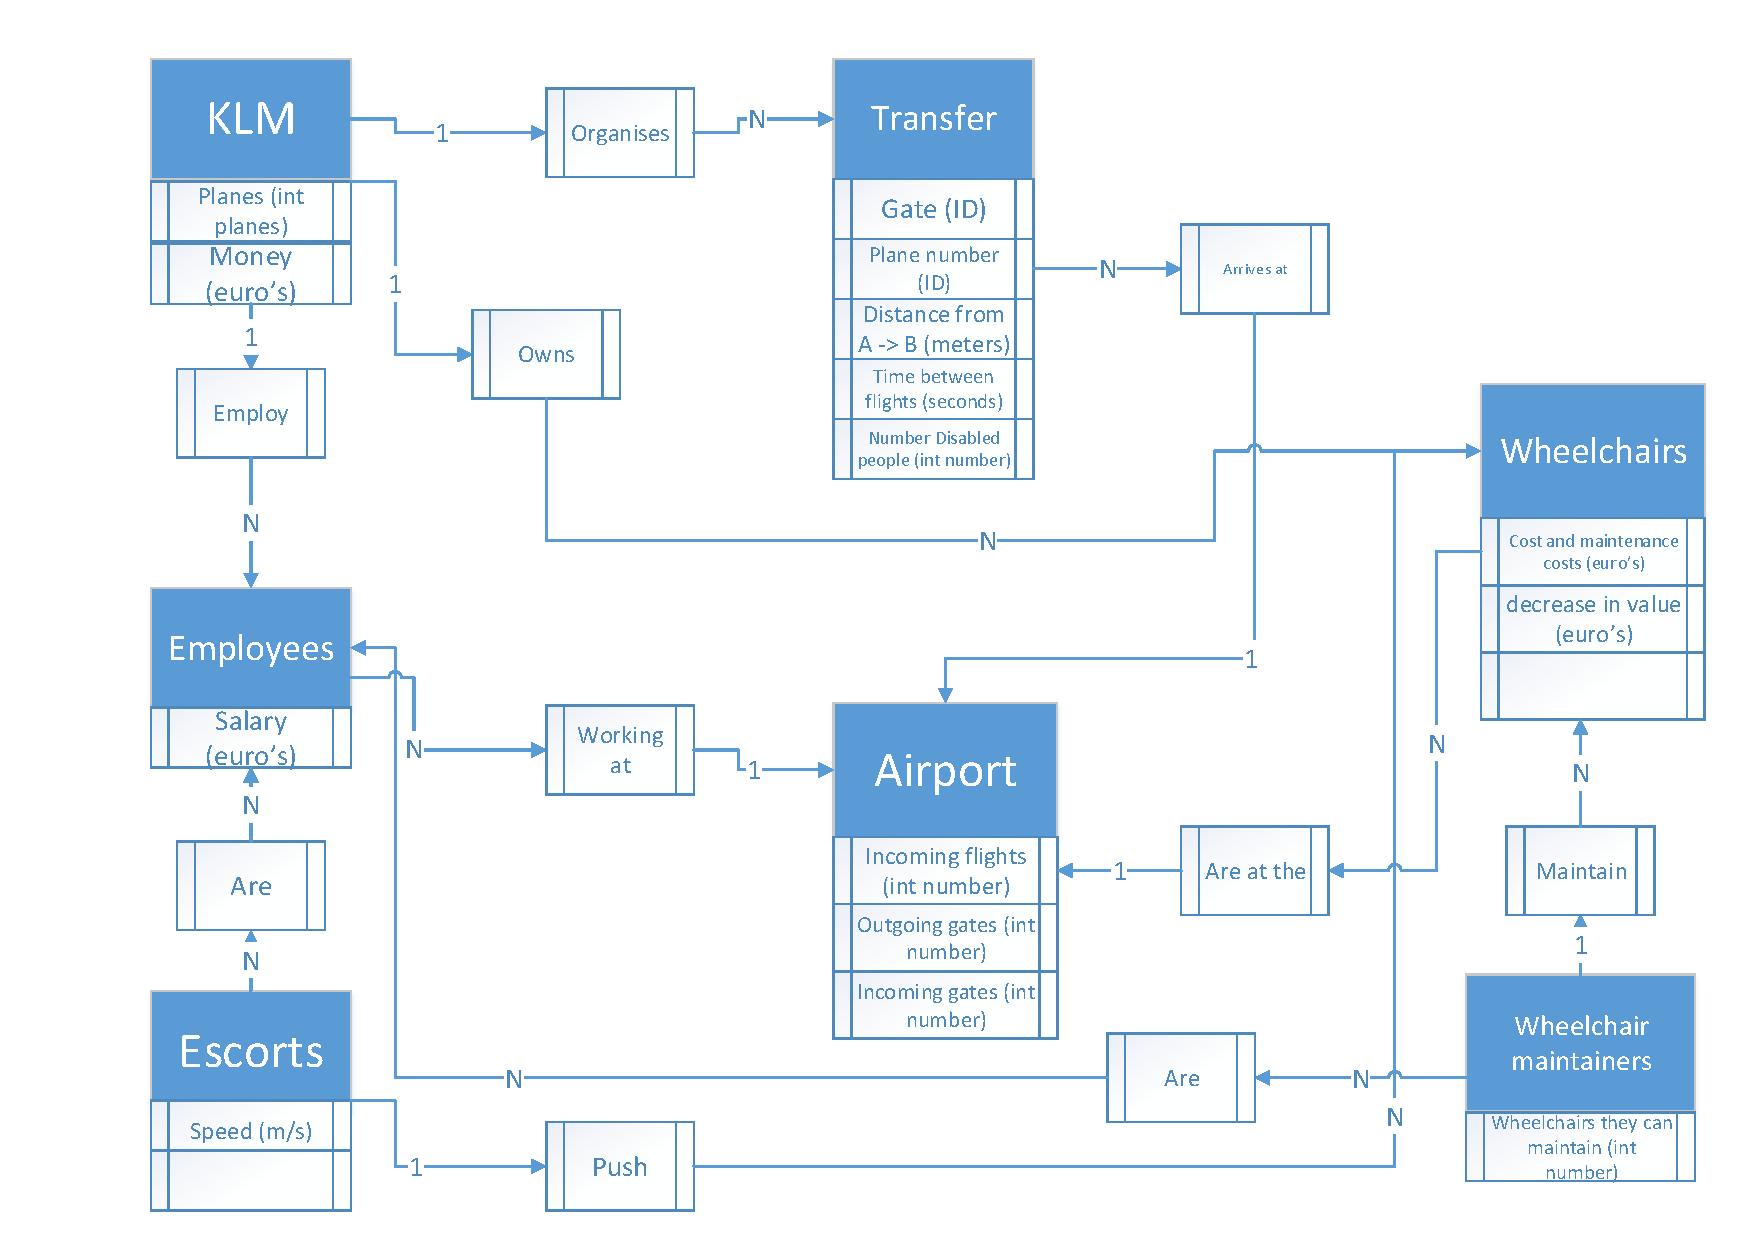
\includegraphics[scale=0.5]{Conceptualmodel.pdf}

\subsection{Explanation of}
\subsubsection{KLM}
The "Money" property is the amount of money KLM has in this model.

\subsubsection{N on N relations of employees, escorts and maintainers}
These are very loose relations. In words this would be: some employees are escorts and some employees are maintainers.

\subsubsection{Time}
There are two values that are described in the unit "euro's/time". This time is not a predetermined value, because it is not known yet in what timeframe we would like to pay them.

\subsubsection{Money}
As one can see, all of the quantities are either usable to determine the eventual amount of money or are already quantified in money.

\chapter{Formalization phase}
\section{Quantities and their relationships}
	\subsection{KLM}
	\begin{description}
	\item[Property:] Money
	\item[Unit:] Euro's
	\item[Role:]
	\end{description}
	\subsection{Employees}
	\begin{description}
	\item[Property:] Salary
	\item[Unit:] Euro's / hour
	\item[Role:]
	\end{description}
	\subsection{Transfer}
	\begin{description}
	\item[Property:] Distance from gate A to B
	\item[Unit:] Meters
	\item[Role:]
	\end{description}
	\begin{description}
	\item[Property:] Time between flights
	\item[Unit:] Seconds
	\item[Role:] To be chosen
	\end{description}
	\begin{description}
	\item[Property:] Disabled people
	\item[Unit:] An integer number
	\item[Role:] To be chosen
	\end{description}
	\subsection{Escorts}
	\begin{Description}
	\item[Property:] Speed
	\item[Unit:] m/s
	\item[Role:] Constant
	\end{Description}
	\subsection{Wheelchairs}
	\begin{Description}
	\item[Property:] Cost and maintenance cost
	\item[Unit:] Euros
	\item[Role:] Constant

	\item[Property:] Decrease in value
	\item[Unit:] Euros/time
	\item[Role:] Constant
	\end{Description}
	\subsection{Wheelchair maintainers}
	\begin{Description}
	\item[Property:] Wheelchairs they can maintain
	\item[Unit:] Integer
	\item[Role:] Constant
	\end{Description}

\section{Approximations and assumptions}
\section{Derivations}
\section{Special cases}
\section{Estimates}

\chapter{Execution phase}
\section{Rephrased problem in formal terms}

%second deadline:
% \section{Quantities and their relationships}
% \section{Approximations and assumptions}
% \section{Derivations}
% \section{Special cases}
% \section{Estimates}

% \chapter{Execution phase}
% \section{Rephrased problem in formal terms}

%third deadline
% \section{Calculation, implementation and simulation}
% \section{Validation and verification; accuracy and precision}

% \chapter{Conclusion phase}
% \section{Presentation and interpretation}

% \chapter{Reflection and discussion}
% \section{Discussion after the conceptual model}
% \section{Discussion after the formal model}
% \section{Discussion after the result}
% \section{Discussion after the solution of the initial problem}

%%%%%%%%% INFORMATION %%%%%%%%%%
% \section{A Note About References}

% The Third and Fourth Year Handbook, and the Third and Fourth Year Project Handbook, have some clear guidelines about plagiarism and referencing.
% You should consult your project supervisor about the correct format for handling references.

% This document uses the `in-text' or Harvard system of referencing, which is a good default format.
% This requires both in-text citations and a list of references at the end of the document.
% The project templates have an example of a list of references.

% Within the text you must cite the authors surname(s) and the date of publication.
% When referring to a specific idea, or a direct quote, you must also give the page number.
% If there are two authors, use `and' and if there are more, use `et al.'\ and give all the authors names at the end.

% There are two styles of citation, implicit and explicit.
% Both are equally acceptable and it is also acceptable to mix and match.

% \subsubsection{Examples of implicit in-text citations}

% The sum of convex functions is itself convex (Blacke, 1985) and therefore any minimiser of this objective function will be a global minimiser (Greene and Whit, 1995, p.123). It is possible to exploit this fact (Browne et al., 2005) to enhance the optimisation algorithm.

% \subsubsection{Examples of explicit in-text citations}

% Blacke (1985) first proved that a sum of convex functions is convex. Any minimiser of this objective function will be a global minimiser, a fact shown by Greene and Whit (1995, p.123) and exploited by Browne et al.\ (2005) to enhance the optimisation algorithm.

%%%%%%%%% APPENDIX %%%%%%%%%%
% \appendix
% \chapter{An Appendix may not be necessary}

% Text introducing the/this appendix.

% \section{Appendix section}

% Text of this section.

% subsubsections and further divisions can also be used in appendices.

%%%%%%%%% BIBLIOGRAPHY %%%%%%%%%%
% \chapter*{Bibliography}

% \begin{description}

% \item Author, I. (Year). \emph{Book Title}, Publisher; Place of publication.

% \item Lamport, L. (1986), \emph{\LaTeX: A Document Preparation System}, Addison-Wesley; Reading, MA.

% \item Author, I. (Year). `Journal article title', \emph{Journal}, \textbf{Vol}, pp.first--last.

% \item Smith, A.D.A.C. and Wand, M.P. (2008). `Streamlined variance calculations for semiparametric
% mixed models', \emph{Statistics in Medicine}, \textbf{27}, pp.435--48.

% \end{description}

\end{document}
